\documentclass[twocolumn]{IEEEtran}
%\documentclass[10pt,graphicx,caption,rotating]{article}
%\textheight=24cm
%\textwidth=17cm
%\topmargin=-2cm
%\oddsidemargin=0cm
\usepackage[utf8x]{inputenc}
\usepackage[activeacute,spanish]{babel}
\usepackage{amssymb,amsfonts}
\usepackage[tbtags]{amsmath}
\usepackage{colortbl}
\usepackage{pict2e}
\usepackage{float}
\usepackage[all]{xy}
\usepackage{graphics,graphicx,color,colortbl}
\usepackage{times}
\usepackage{subfigure}
\usepackage{wrapfig}
\usepackage{multicol}
\usepackage{colortbl}
\usepackage{cite}
\usepackage{url}
\usepackage[tbtags]{amsmath}
\usepackage{amsmath,amssymb,amsfonts,amsbsy}
\usepackage{bm}
\usepackage{algorithm}
\usepackage{algorithmic}
\usepackage{listings}
\usepackage[centerlast, small]{caption}
\usepackage[colorlinks=true, citecolor=blue, linkcolor=blue, urlcolor=blue, breaklinks=true]{hyperref}
\begin{document}
\title{\huge{Estudio fotográfico semi-profesional}}
\author{David Ricardo Martínez Hernández Código: $261931$\\
	Juan Sebastian Roncancio Arevalo Código: $261585$}
\date{}
\maketitle
\floatname{algorithm}{Algoritmo}

\section{Introducción}
\noindent
Este documento contiene el proceso de diseño e implementación del estudio fotográfico aficionado, se ha realizado un trabajo a lo largo del semestre en la manipulación de motores, iluminación y visualización a través de procesador indicado para el curso, este desarrollo tomo varias consideraciones al igual que cambios y reformas a medida que se iba avanzando, el desarrollo del proyecto utilizo una metodología top-down en la que se partían de ideas abstractas y a medida que se iban concretando se iban especificando cada vez mas hasta llegar al punto en que se consideraba era el prototipo final.\\
La fotografía ha consolidado a través de la historia la mejor forma de capturar e inmortalizar momentos y situaciones, gracias a esta técnica hemos conocido importantes pasajes de la historia, esto ha ayudado al desarrollo y evolución de nuestra sociedad. También ha sido de gran aporte en las áreas militares y científicas, además su goce y disfrute hace que emerja una gran pasión para algunas personas que encuentran en esta práctica su estilo de vida.\\
Se debe recordemos que la acción de inmortalizar momentos viene desde nuestros ancestros que disfrutaban el arte de plasmar dichos momentos en las paredes ``jeroglífico'' ó dejando imágenes en libros o manuscritos, los cuales han sido el primer paso para muchas investigaciones y avances significativos para la sociedad.\\
Teniendo en cuenta que la fotografía ha tomando gran importancia se desarrolló un estudio semi-profesional, con el fin de hacer más fácil la realización de esta práctica. Se controlaron algunos aspectos sencillos, con los cuales el usuario puede establecer las condiciones a su gusto, para así mejorar la experiencia de la captura desde cualquier ángulo y contrastes preferidos.\\
Como se ha logrado ver estudios especializados este tipo de estudios no han tenido un gran auge, puesto que dicha clase de estudios solo están al alcance de personas de un alto puesto en la sociedad o poder de adquisición. Este es un sistema automatizado de fotografía similar a los estudios profesionales para que puedan ser adquiridos por un mayor número de personas y así esta profesión sea popularizada.

\section{Objetivos}
\subsection{General}
\begin{itemize}
 \item Desarrollar un estudio semi-profesional de Fotografía, tomando como cámara dispositivo con Bluetooth.
\end{itemize}

\subsection{Específicos}
\begin{itemize}
 \item Realizar el control de los motores por medio de unos interruptores, con dos grados de libertad.
 \item Generar un periférico para el procesador LM32.
 \item Realizar una visualización por medio de una LCD, para llevar el control todo el control del estudio.
\end{itemize}

\section{Secuencia y tipo de actividades que se desarrollaron}
\noindent
\begin{enumerate}
 \item Control y el correcto funcionamiento de los motores para las lamparas y la silla.
 \item Construcción de las lamparas y de la silla.
 \item Implementación del periférico para el procesador LM32.
 \item Control de la intensidad de las luces.
\end{enumerate}

\section{Cronograma}
\noindent
El tiempo en el cual se realizaron las tareas se puede apreciar en el TABLA \ref{tab1}.
\begin{table}[H]
	\centering
\begin{tabular}{|c|c|c|c|c|}\hline
Semanas & Control Motores & Lampara y Silla & Periférico & Luces \\ \hline
2 & & & & \\ \hline
3 & & & & \\ \hline
4 & & & & \\ \hline
5 & & & & \\ \hline
6 & & & & \\ \hline
7 & & & & \\ \hline
8 & & & & \\ \hline
9 & & & & \\ \hline
10 & & & & \\ \hline
11 & \cellcolor{black} & & & \\ \hline
12 & \cellcolor{black} & & & \\ \hline
13 & \cellcolor{black} & \cellcolor{black} & & \cellcolor{black} \\ \hline
14 & \cellcolor{black} & \cellcolor{black} & \cellcolor{black} & \cellcolor{black} \\ \hline
15 & \cellcolor{black} & \cellcolor{black} & \cellcolor{black} & \cellcolor{black} \\ \hline
16 & & & & \\ \hline
    \end{tabular}
	\caption{Cronograma de actividades que se realizo}
	\label{tab1}
\end{table}
\noindent
Como se puede observar en el TABLA \ref{tab2}, el cronograma vario, se esperaba terminar algunas tareas en un menor tiempo pero todos las tareas empezaron a tomar un tiempo mayor de realización, esto conllevo a que se acumularan otras tareas.
\begin{table}[H]
	\centering
\begin{tabular}{|c|c|c|c|c|}\hline
Semanas & Control Motores & Lampara y Silla & Periférico & Luces \\ \hline

2 & & & & \\ \hline
3 & & & & \\ \hline
4 & & & & \\ \hline
5 & & & & \\ \hline
6 & & & & \\ \hline
7 & & & & \\ \hline
8 & & & & \\ \hline
9 & \cellcolor{black} & & & \\ \hline
10 & \cellcolor{black} & \cellcolor{black} & & \\ \hline
11 & & \cellcolor{black} & & \\ \hline
12 & & \cellcolor{black} & \cellcolor{black} & \\ \hline
13 & & & \cellcolor{black} & \cellcolor{black} \\ \hline
14 & & & & \cellcolor{black} \\ \hline
15 & & & & \\ \hline
16 & & & & \\ \hline
    \end{tabular}
	\caption{Cronograma propuesto para desarrollar las actividades}
	\label{tab2}
\end{table}
\noindent
La construcción de la lampara y de la silla se atraso porque no se habían podido comprar los motores dado que no se tenia el dinero suficiente, a los motores se les hizo un buje para poder adaptarlos a la estructura.\\

\section{Comportamiento}
\noindent
El desarrollo del proyecto consiste en  un estudio fotográfico aficionado versátil. Debido al avance tecnológico creemos que los Smartphones pueden llegar a reemplazar las cámaras fotográficas dirigidas a usuarios aficionados, por esta razón se impulso el desarrollo de este prototipo.
Este prototipo cuenta con una lámpara y una silla central la cual se usa como un dispositivo donde se ubicaran los objetos que serán fotografiados; idea de esta silla es que el objeto gire sobre un eje central, de manera que se tenga la posibilidad de encontrar el mejor ángulo fotográfico al tomarse varias tomas.\\

\subsection{Limitaciones}
\noindent
Al haber terminado por completo la estructura de la lampara nos dimos cuenta que el motor superior de la lampara no era lo suficientemente poderoso para sostener el buje de adaptación y la ``L'' que se conecta a las luces, esa es una limitación que tiene el montaje.\\
La no implementación de las luces a partir del se considerara  una limitación importante; si bien está que se ahorran recursos de ejecución  y operación, también se debe tener en cuenta que el reto era poder controlar todo desde el procesador.\\
Debido al gran costo de la construcción de las lámparas y del precio de cada motor sólo se presenta una lámpara y la silla central, Sin embargo, el desarrollo del dispositivo para lámparas adicionales se puede efectuar a partir del implementado actualmente. Consideramos que esta es una limitación mínima pues esta implementación  se limita única y exclusivamente a recursos económicos.

\section{Arquitectura Y Estructura}
\noindent
En la figura 1 se muestra una estructura general del proyecto. A medida que se avanza en el informe se irá haciendo un acercamiento a cada uno de los bloques ilustrados en la Fig. \ref{fig1}
\begin{figure}[H]
	\centering
		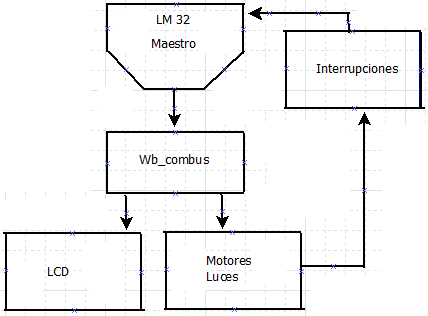
\includegraphics[scale=0.5]{Structure.png}
	\caption{Estructura Del Proyecto}
	\label{fig1}
\end{figure}

\subsection{Hardware}
\noindent
Al inicio del desarrolló se determinaron  criterios para dividir las tareas a efectuarse en hardware y software.  Se puede entender por hardware como todo aquello que es tangible, de manera que se instancian los módulos de los motores y las luces como tareas de este tipo. Por otro lado, software es aquello que no tiene relación directa con el usuario, pero que efectúa operaciones internas; debido a esto se ha decidido que el manejo de la LCD y el control general del dispositivo sea una tarea que corresponda al desarrollo software. En forma gráfica el proyecto se dispone como se muestra en la Fig. \ref{fig2}.
\begin{figure}[H]
	\centering
		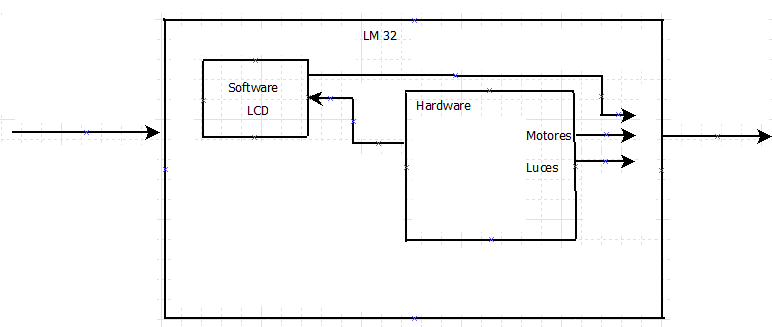
\includegraphics[scale=0.3]{architecture.png}
	\caption{Arquitectura General}
	\label{fig2}
\end{figure}

\subsection{Motores}
\noindent
Para el desarrollo de este prototipo se usaron motores paso – paso unipolares. El control de dichos motores se realizó en lenguaje de descripción de hardware y su funcionamiento es basado en el envió de  pulsos de 4 bits en forma secuencial. Estos elementos mecánicos se componen de 4 bobinas (correspondiendo cada bit a una de estas bobinas), de manera que los pulsos enviados activan  las bobinas por pares, de esta forma dan movimiento a los motores. Este proceso se muestra en la siguiente Fig. \ref{fig3}.
\begin{figure}[H]
	\centering
		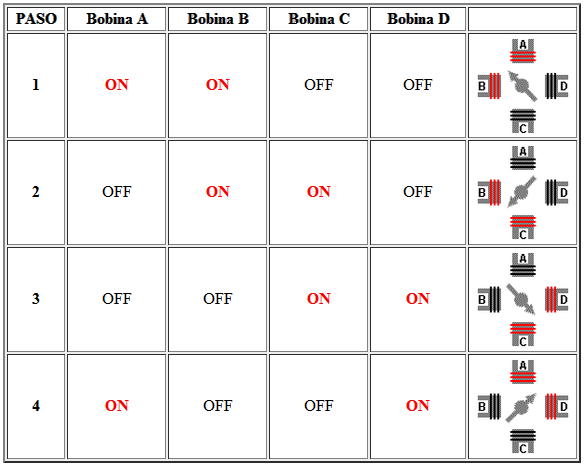
\includegraphics[scale=0.4]{secuence.png}
	\caption{Secuencia de Conexión de los motores}
	\label{fig3}
\end{figure}
\noindent
Al implementar la tabla que se muestra en la Fig. \ref{fig3} en un lenguaje HDL obtenemos el siguiente modulo, este modulo ilustrado en la Fig. \ref{fig4}, contiene todas las señales de control necesarias para la manipulación de los cinco motores.
\begin{figure}[H]
	\centering
		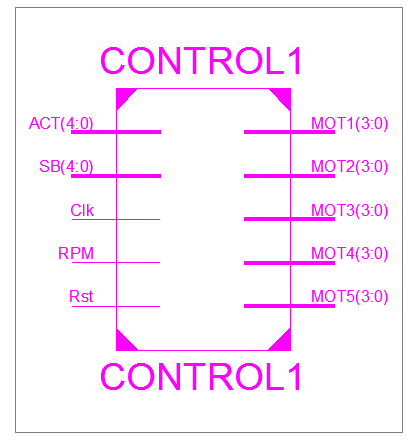
\includegraphics[scale=0.4]{control.png}
	\caption{Control de los motores}
	\label{fig4}
\end{figure}
\noindent
El módulo  tiene $5$ señales de control denominadas en su respectivo orden de la siguiente manera:
\begin{itemize}
 \item ACT: la cual nos permite encender o apagar el motor.
 \item SB: permite controlar la dirección del giro del motor.
 \item ClK: controla el movimiento del motor ya que todos se realizan en torno a divisores de frecuencia.
 \item RPM: permite seleccionar la velocidad de giro del motor.
 \item Rst: una señal que proporciona un restablecimiento a un estado predeterminado.
 \end{itemize}
\noindent
En esta tarea se controlan los cinco motores y cada uno ellos responde de la misma manera ante las señales mencionadas anteriormente.
\begin{figure}[H]
	\centering
		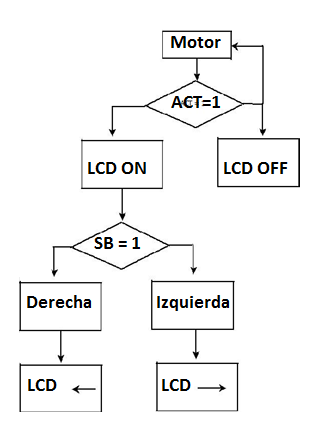
\includegraphics[scale=0.5]{control2.png}
	\caption{Diagrama de Flujo de los motores}
	\label{fig5}
\end{figure}
\noindent
Adicional al control realizado en la tarjeta de desarrollo, los motores cuentan con un circuito externo, conocidos popularmente como puente H. Estos circuitos proveen al motor una alimentación externa evitando así que se le pida a la tarjeta de desarrollo tensiones o corrientes por encima de los valores normales con los que ellas trabajan, para dicho montaje se uso el CI UNL $2803$ y una $L7805$, el cual regula la tensión para que el CI trabaje sin mucho esfuerzo. El circuito externo para dicha función se presenta en la Fig. \ref{fig6}.
\begin{figure}[H]
	\centering
		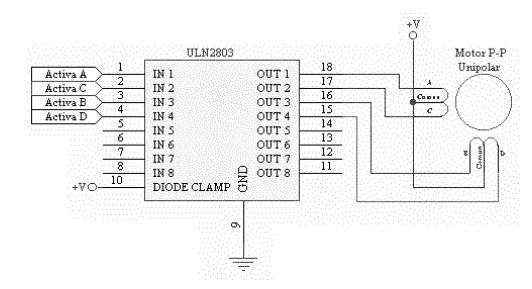
\includegraphics[scale=0.5]{esquematico.png}
	\caption{Esquemático del Puente H a los motores}
	\label{fig6}
\end{figure}

\subsection{Luces}
\noindent
Las luces usadas para este dispositivo son versátiles y económicas, y se alimentan con  una fuente DC, con tensión de alimentación es $12$ V.  Su iluminación al ser tecnología led proporciona un desempeño mejor que al usar lámparas incandescentes. Se pretendía controlar las lámparas con un modulo de PWM, sin embargo logro poner en práctica debido a que la etapa de potencia necesaria para hacer funcionar dicho circuito aun no está a nuestro alcance, pero se desarrollo un pequeño circuito que controla  otros leds  de una potencia e intensidad más baja para hacer la prueba de que dicho modulo si se implemento solo que la alimentación externa no se pudo determinar.\\
Para corregir esta falla se diseñó un circuito donde la alimentación de las lámparas fuese tomada directamente de la fuente. Esto proporciona dos ventajas adicionales:
\begin{enumerate}
 \item Se economizan recursos pues el control de la luces es más simple
 \item Es posible alcanzar una calidad de luces mucho mejor ya que la lámparas de los estudios profesionales son muy potentes y su consumo de energía es alto, con esto simplemente se economizan recursos de construcción y gastos de operación.
\end{enumerate}
\begin{figure}[H]
	\centering
		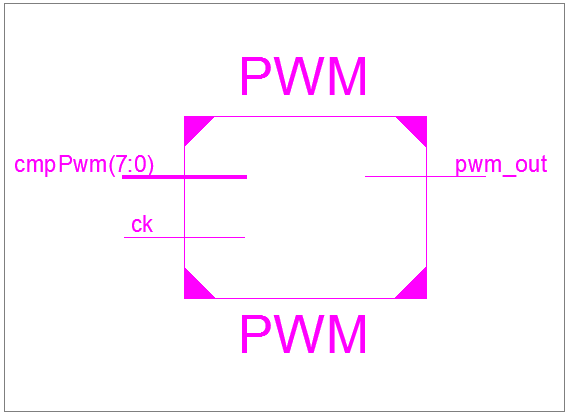
\includegraphics[scale=0.45]{pwm.png}
	\caption{Configuración para el PWM}
	\label{fig7}
\end{figure}
\noindent
Para el diseño de las lámparas controladas desde la FPGA el bloque de las luces se muestra en la Fig. \ref{fig7}, para este modulo solo se tendrían dos señales de control.\\
\begin{itemize}
 \item cmpPwm de 8 bits la cual está encargada de controlar el valor medio de la señal de salida.
 \item ck que es el reloj de la FPGA.
\end{itemize}

\subsection{LCD}
\noindent
Este periférico permite al usuario observar el estado de cada motor. En esta se muestra si los elementos están encendidos (ON), apagados (OFF) y además su sentido de giro, ya sea en sentido horario ($->$) o anti-horario ($<-$).  El esquema del módulo se aprecia en la Fig. \ref{fig8}
\begin{figure}[H]
	\centering
		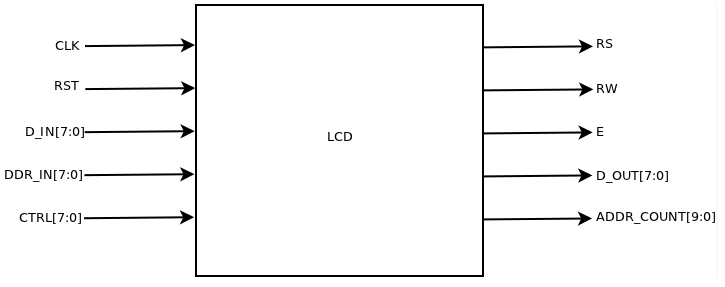
\includegraphics[scale=0.45]{lcd.png}
	\caption{Diagrama esquemático del LCD}
	\label{fig8}
\end{figure} 
\noindent
El control del periférico se efectúa como tarea software, en donde se realizan los procesos de la inicialización y la lectura de datos por parte de la LCD. El funcionamiento se ilustra en la Fig. \ref{fig9}
\begin{figure}[H]
	\centering
		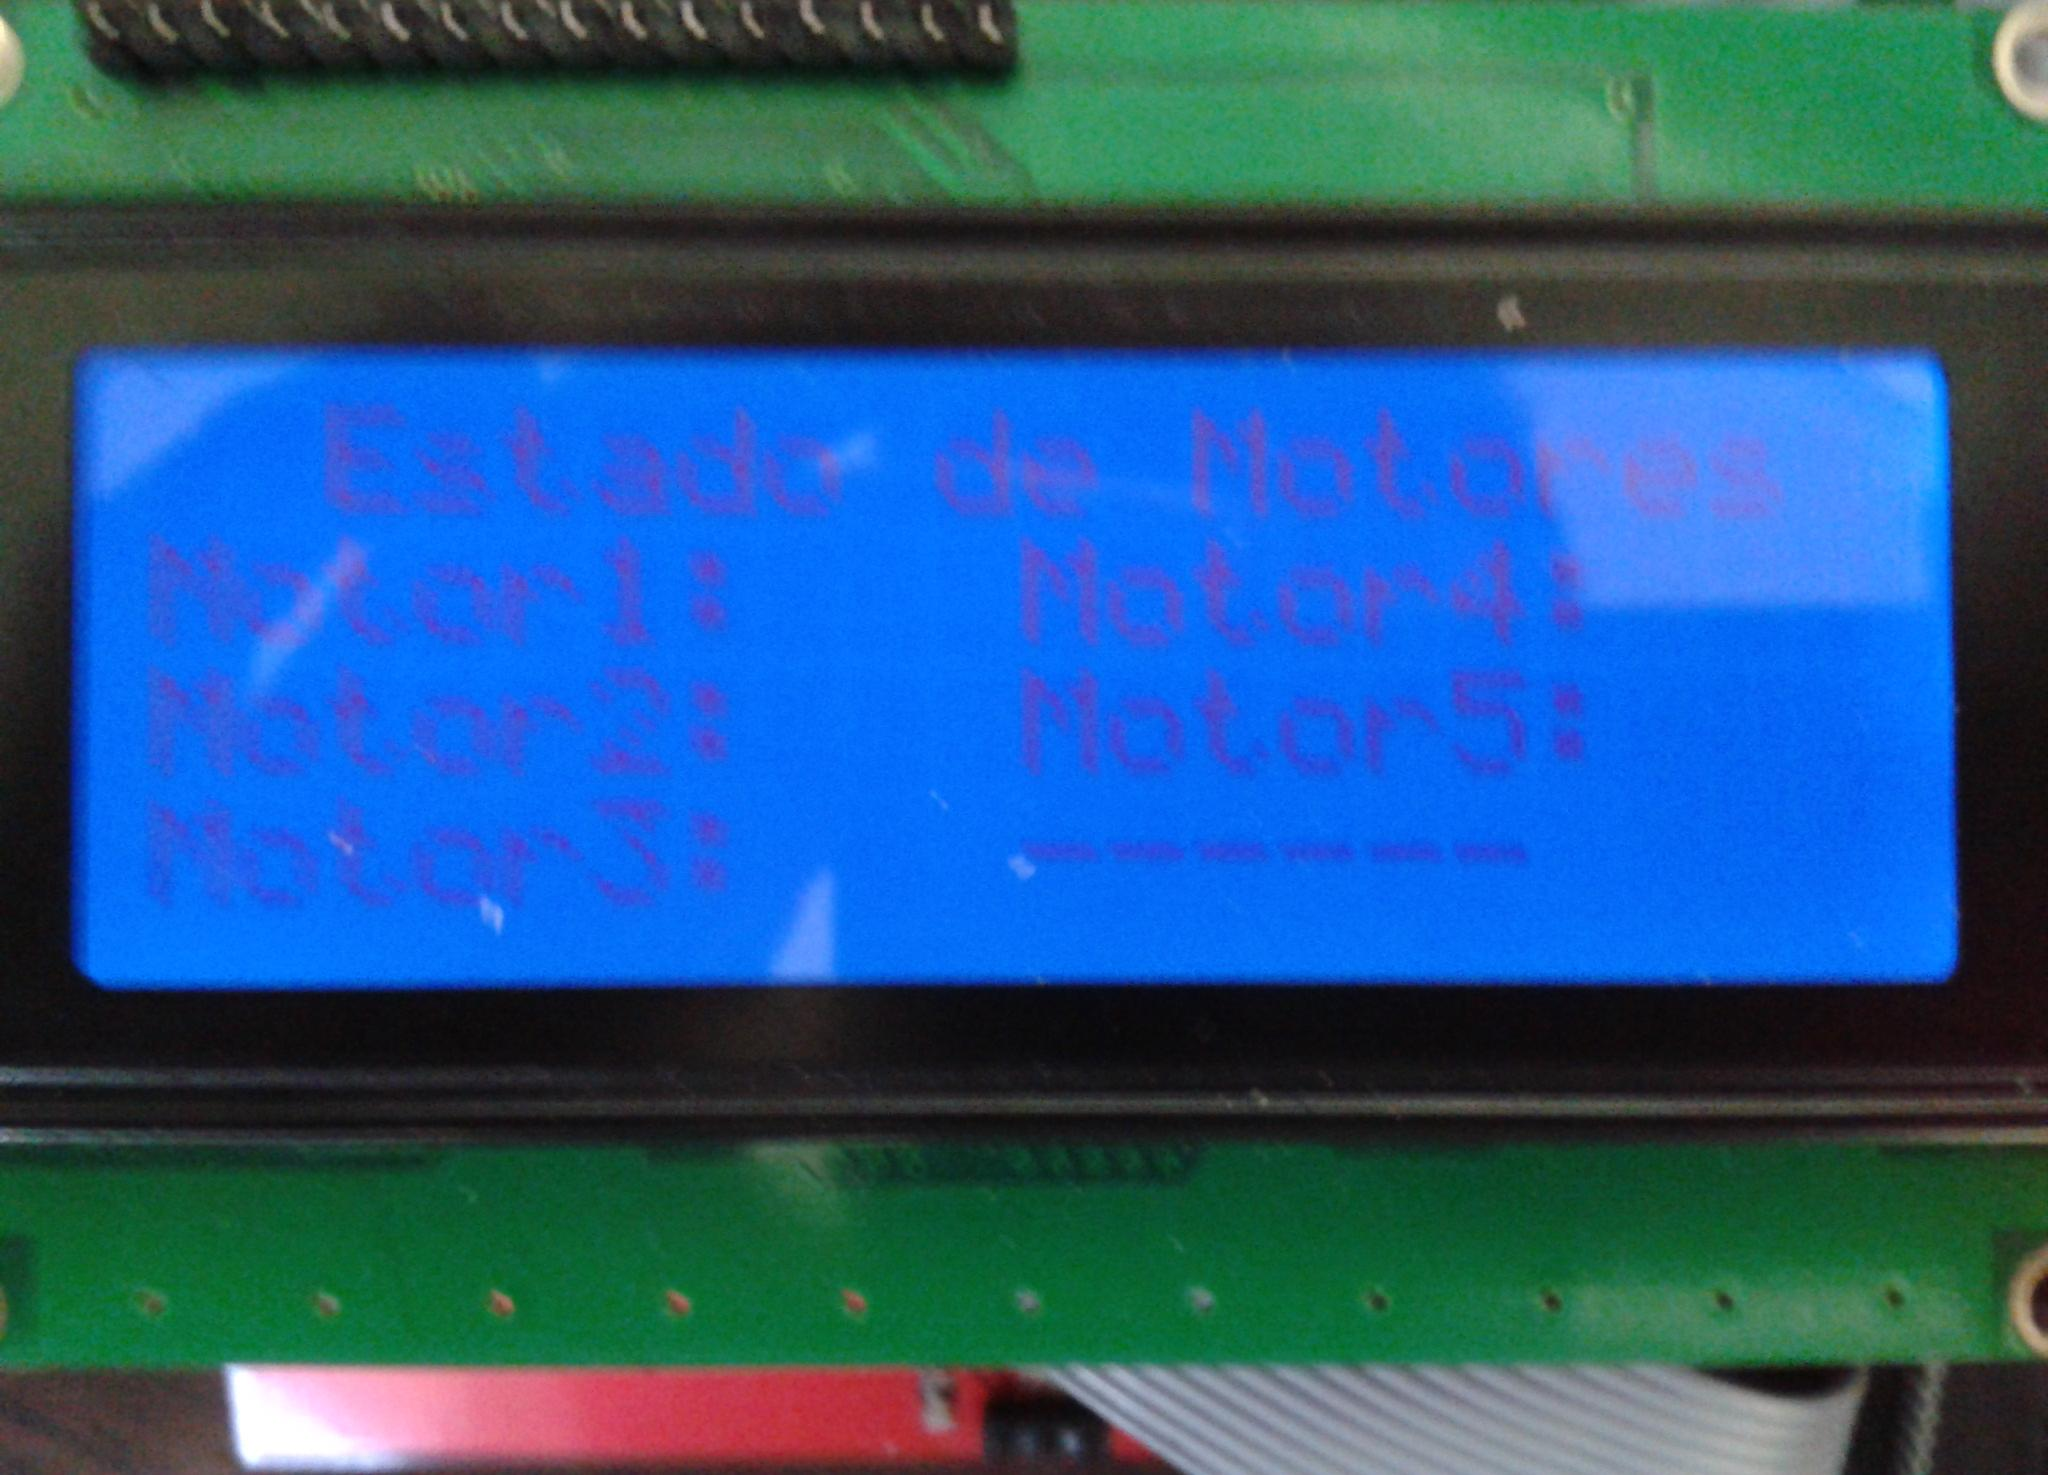
\includegraphics[scale=0.15]{lcd2.png}
	\caption{LCD funcionando}
	\label{fig9}
\end{figure} 

\section{Análisis Económico}
\noindent
Para realizar la estructura de la lampara y de la silla se compro un tubo de $5/32'$, una hoja de segueta para realizar los cortes, una broca de $1/8'$, las bases circulares para los motores, estos materiales se llevaron a donde un soldador para que armara la estructura y se le hicieron los huecos para los pasadores de aseguramiento. Se fue a donde una persona que manejara un torno industrial para que realizara los bujes de adaptación del los motores a la estructura. Al tener todo esto ya terminado se comenzó con el armado final, lo primero que se hizo fue abrir los huecos a los soportes metálicos de los motores para asegurarlos a las estructuras con una broca de $3/4'$, los tornillos, las arandelas y las tuercas, se pintaron las piezas con la laca y finalmente se acoplaron los motores a la estructura. Para la base de la silla se le abrieron los huecos que aseguraban la base cuadrada con la base circular de madera con una broca de $3/4'$, se aseguraron con los tornillos y tuercas. Se pego la cinta de decoración a la base de madera. Por el costo  tan elevado de las estructuras se decidió realizar una sola lampara y una silla.

\begin{table}[H]
	\centering
\begin{tabular}[c]{|c|c|c|c|} \hline
\textbf{Materiales} & \textbf{Valor} & \textbf{Unidades} & \textbf{Costo} \\ \hline
Broca de $1/8'$ & $2000$ & $1$ & $2000$ \\%pines
Broca de $3/16'$ & $2000$ & $1$ & $2000$ \\%Huecos motores
Tornillos, Arandelas y Tuercas Cincados & $200$ & $15$ & $3000$ \\
Tubo de $5/32$ Calibre 18 & $15000$ & $1$ & $15000$ \\
Pintura en laca & $12000$ & $1$ & $15000$ \\ 
Base circular Calibre 16 & $2000$ & $2$ & $4000$ \\
Base de madera & $2000$ & $1$ & $2000$ \\
Bujes de adaptación Motores-Tubo  & $15000$ & $3$ & $45000$ \\
Mano de obra soldadura & $20000$ & $1$ & $20000$ \\
Base cuadrada Calibre $18$ Colrol & $2000$ & $1$ & $2000$ \\
Cinta cobertura base circular & $1000$ & $1$ & $1000$ \\
Hoja de segueta & $3000$ & $1$ & $3000$ \\
LCD & $35000$ & $1$ & $35000$ \\
Motores & $15000$ & $3$ & $45000$ \\
Circuitos Impresos & $14000$ & $5$ & $70000$ \\
Potenciómetros & $500$ & $2$ & $1000$ \\
Resistencias & $100$ & $27$ & $2700$ \\
Switch & $700$ & $12$ & $8400$ \\
LED's & $300$ & $27$ & $8100$ \\
Caja & $10000$ & $1$ & $1000$ \\
FPGA & $250000$ & $1$ & $250000$ \\
Conexiones & $7000$ & $1$ & $7000$ \\
Mano de Obra Ingenieros & $30000$ & $128$ & $3480000$\\ \hline
\textbf{Total} &  &  & $4028200$ \\ \hline
\end{tabular}
	\caption{Tabla de costos de los materiales utilizados}
	\label{tabcosto}
\end{table}



\section{Conclusiones}
\begin{itemize}
 \item Al iniciar el desarrollo del proyecto no se tenía una estructura clara de lo que se quería hacer por lo tanto todo se desarrollaba de forma lineal, en el momento en que empezamos a tener problemas nos dimos cuenta que debíamos reestructuras nuestro diseño y partir con metodologías top-dowm, que  permite  especificar el funcionamiento y estructura de los diseños.
 \item Luego de revisar alguna teoría sobre los motores nos encontramos con algo que produjo gran controversia, pues estos motores también pueden ser controlados por módulos de PWM, sin embargo debido al tiempo y proceso de diseño que llevábamos en el momento de conocer esta forma decidimos continuar con nuestro desarrollo como se tenía pensado desde el comienzo.
 \item Dado que los elementos que se compraron son de medida estándar fue muy complicado e inesperado hacer las adaptaciones mecánicas necesarias para que se pudiera adecuar a los requerimientos del proyecto, por ejemplo los bujes de adaptación para los motores y la estructura, fue muy complicado lelgar a la solución del problema.
\end{itemize}
\bibliographystyle{ieeetran}
\begin{thebibliography}{99}
\bibitem{page1} Sitio Web: \url{http://www.todorobot.com.ar/informacion/tutorial%20stepper/stepper-tutorial.htm}
\end{thebibliography}
\end{document}